\definecolor{aa}{rgb}{0.00000   0.44700   0.74100}
\definecolor{ab}{rgb}{0.85000   0.32500   0.09800}
\definecolor{ac}{rgb}{1.00000   0.00000   1.00000}
\definecolor{ak}{RGB}{0,0,0}

% GNUPLOT: LaTeX picture with Postscript
\begingroup
  \makeatletter
  \providecommand\color[2][]{%
    \GenericError{(gnuplot) \space\space\space\@spaces}{%
      Package color not loaded in conjunction with
      terminal option `colourtext'%
    }{See the gnuplot documentation for explanation.%
    }{Either use 'blacktext' in gnuplot or load the package
      color.sty in LaTeX.}%
    \renewcommand\color[2][]{}%
  }%
  \providecommand\includegraphics[2][]{%
    \GenericError{(gnuplot) \space\space\space\@spaces}{%
      Package graphicx or graphics not loaded%
    }{See the gnuplot documentation for explanation.%
    }{The gnuplot epslatex terminal needs graphicx.sty or graphics.sty.}%
    \renewcommand\includegraphics[2][]{}%
  }%
  \providecommand\rotatebox[2]{#2}%
  \@ifundefined{ifGPcolor}{%
    \newif\ifGPcolor
    \GPcolorfalse
  }{}%
  \@ifundefined{ifGPblacktext}{%
    \newif\ifGPblacktext
    \GPblacktexttrue
  }{}%
  % define a \g@addto@macro without @ in the name:
  \let\gplgaddtomacro\g@addto@macro
  % define empty templates for all commands taking text:
  \gdef\gplfronttext{}%
  \gdef\gplfronttext{}%
  \makeatother
  \ifGPblacktext
    % no textcolor at all
    \def\colorrgb#1{}%
    \def\colorgray#1{}%
  \else
    % gray or color?
    \ifGPcolor
      \def\colorrgb#1{\color[rgb]{#1}}%
      \def\colorgray#1{\color[gray]{#1}}%
      \expandafter\def\csname LTw\endcsname{\color{white}}%
      \expandafter\def\csname LTb\endcsname{\color{black}}%
      \expandafter\def\csname LTa\endcsname{\color{black}}%
      \expandafter\def\csname LT0\endcsname{\color[rgb]{1,0,0}}%
      \expandafter\def\csname LT1\endcsname{\color[rgb]{0,1,0}}%
      \expandafter\def\csname LT2\endcsname{\color[rgb]{0,0,1}}%
      \expandafter\def\csname LT3\endcsname{\color[rgb]{1,0,1}}%
      \expandafter\def\csname LT4\endcsname{\color[rgb]{0,1,1}}%
      \expandafter\def\csname LT5\endcsname{\color[rgb]{1,1,0}}%
      \expandafter\def\csname LT6\endcsname{\color[rgb]{0,0,0}}%
      \expandafter\def\csname LT7\endcsname{\color[rgb]{1,0.3,0}}%
      \expandafter\def\csname LT8\endcsname{\color[rgb]{0.5,0.5,0.5}}%
    \else
      % gray
      \def\colorrgb#1{\color{black}}%
      \def\colorgray#1{\color[gray]{#1}}%
      \expandafter\def\csname LTw\endcsname{\color{white}}%
      \expandafter\def\csname LTb\endcsname{\color{black}}%
      \expandafter\def\csname LTa\endcsname{\color{black}}%
      \expandafter\def\csname LT0\endcsname{\color{black}}%
      \expandafter\def\csname LT1\endcsname{\color{black}}%
      \expandafter\def\csname LT2\endcsname{\color{black}}%
      \expandafter\def\csname LT3\endcsname{\color{black}}%
      \expandafter\def\csname LT4\endcsname{\color{black}}%
      \expandafter\def\csname LT5\endcsname{\color{black}}%
      \expandafter\def\csname LT6\endcsname{\color{black}}%
      \expandafter\def\csname LT7\endcsname{\color{black}}%
      \expandafter\def\csname LT8\endcsname{\color{black}}%
    \fi
  \fi
    \setlength{\unitlength}{0.0500bp}%
    \ifx\gptboxheight\undefined%
      \newlength{\gptboxheight}%
      \newlength{\gptboxwidth}%
      \newsavebox{\gptboxtext}%
    \fi%
    \setlength{\fboxrule}{0.5pt}%
    \setlength{\fboxsep}{1pt}%
\hspace{1cm}
\begin{picture}(7000.00,7000.00)%
    \gplgaddtomacro\gplfronttext{%
      \colorrgb{0.15,0.15,0.15}%
      \put(600,2189){\makebox(0,0)[r]{\strut{}$6.0$}}%
      \colorrgb{0.15,0.15,0.15}%
      \put(600,2784){\makebox(0,0)[r]{\strut{}$8.0$}}%
      \colorrgb{0.15,0.15,0.15}%
      \put(600,3378){\makebox(0,0)[r]{\strut{}$10.0$}}%
      \colorrgb{0.15,0.15,0.15}%
      \put(600,3973){\makebox(0,0)[r]{\strut{}$12.0$}}%
      \colorrgb{0.15,0.15,0.15}%
      \put(600,4567){\makebox(0,0)[r]{\strut{}$14.0$}}%
      \colorrgb{0.15,0.15,0.15}%
      \put(600,5162){\makebox(0,0)[r]{\strut{}$16.0$}}%
      \colorrgb{0.00,0.00,0.00}%
      \put(940,1880){\makebox(0,0){\strut{}$-2.0$}}%
      \colorrgb{0.00,0.00,0.00}%
      \put(1535,1880){\makebox(0,0){\strut{}$0.0$}}%
      \colorrgb{0.00,0.00,0.00}%
      \put(2129,1880){\makebox(0,0){\strut{}$2.0$}}%
      \colorrgb{0.00,0.00,0.00}%
      \put(2724,1880){\makebox(0,0){\strut{}$4.0$}}%
      \colorrgb{0.00,0.00,0.00}%
      \put(3318,1880){\makebox(0,0){\strut{}$6.0$}}%

      \put(1820,5804){\makebox(0,0){\strut{}{\color{ak}{\rule[0.6mm]{0.5cm}{0.5mm}}} Τροχιά αισθητήρα}}
      \put(4500,6204){\makebox(0,0){\strut{} Εκτιμώμενη τροχιά μέσω}}
      \put(3570,5804){\makebox(0,0){\strut{}{\color{aa}{\rule[0.6mm]{0.5cm}{0.5mm}}} PLICP}}
      \put(4700,5804){\makebox(0,0){\strut{}{\color{ab}{\rule[0.6mm]{0.5cm}{0.5mm}}} NDT}}
      \put(5740,5804){\makebox(0,0){\strut{}{\color{ac}{\rule[0.6mm]{0.5cm}{0.5mm}}} \texttt{fsm}}}
      \put(-100,4300){\rotatebox{90}{\makebox(0,0)[r]{\strut{}$\sigma_R = 0.0$ m}}}%
    }%
    \gplgaddtomacro\gplfronttext{%
    }%
    \gplgaddtomacro\gplfronttext{%
      \colorrgb{0.00,0.00,0.00}%
      \put(3950,1880){\makebox(0,0){\strut{}$-2.0$}}%
      \colorrgb{0.00,0.00,0.00}%
      \put(4544,1880){\makebox(0,0){\strut{}$0.0$}}%
      \colorrgb{0.00,0.00,0.00}%
      \put(5139,1880){\makebox(0,0){\strut{}$2.0$}}%
      \colorrgb{0.00,0.00,0.00}%
      \put(5733,1880){\makebox(0,0){\strut{}$4.0$}}%
      \colorrgb{0.00,0.00,0.00}%
      \put(6327,1880){\makebox(0,0){\strut{}$6.0$}}%
    }%
    \gplgaddtomacro\gplfronttext{%
    }%
    \put(0,0){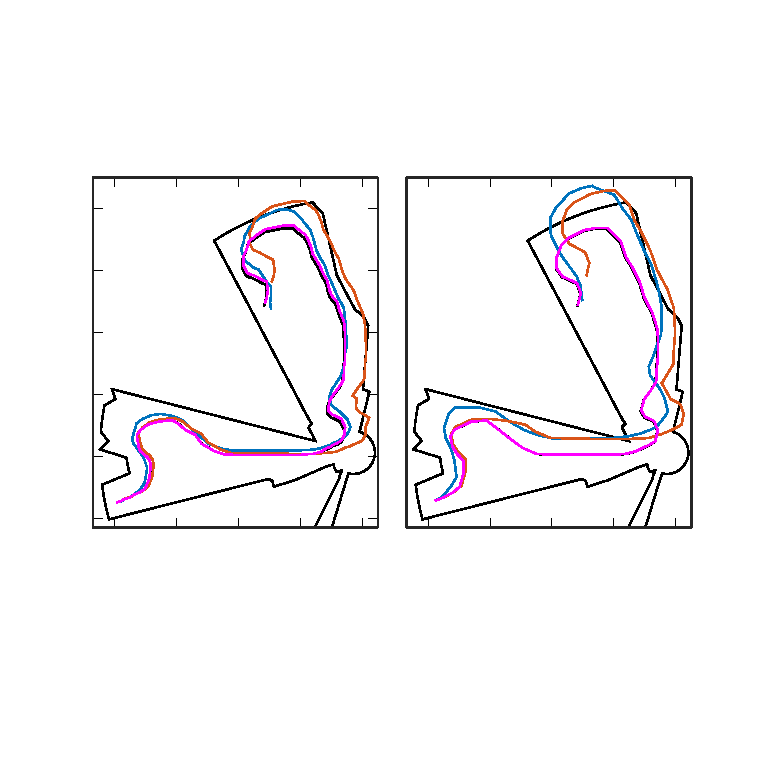
\includegraphics{./figures/parts/02/chapters/05/sections/04/odom_test_5_vs_6_sr_000}}%
    \gplfronttext
  \end{picture}%
\endgroup
